% Sidst opdateret: 25/1 1994
\documentstyle[a4,nfdcfnt,12pt]{article}
% Psfig/TeX Release 1.2
%
% Archive users note: this is an out-of-date version, preserved because future
% versions are backwards incompatible. Use psfig.sty for the up-to-date
% version.
%
% dvips version
%
% All software, documentation, and related files in this distribution of
% psfig/tex are Copyright 1987, 1988 Trevor J. Darrell
%
% Permission is granted for use and non-profit distribution of psfig/tex 
% providing that this notice be clearly maintained, but the right to
% distribute any portion of psfig/tex for profit or as part of any commercial
% product is specifically reserved for the author.
%
% $Header: psfig.tex,v 1.9 88/01/08 17:42:01 trevor Exp $
% $Source: $
%
% Thanks to Greg Hager (GDH) and Ned Batchelder for their contributions
% to this project.
%
\catcode`\@=11\relax
\newwrite\@unused
\def\typeout#1{{\let\protect\string\immediate\write\@unused{#1}}}
\typeout{psfig/tex 1.2-dvips}


%% Here's how you define your figure path.  Should be set up with null
%% default and a user useable definition.

\def\figurepath{./}
\def\psfigurepath#1{\edef\figurepath{#1}}

%
% @psdo control structure -- similar to Latex @for.
% I redefined these with different names so that psfig can
% be used with TeX as well as LaTeX, and so that it will not 
% be vunerable to future changes in LaTeX's internal
% control structure,
%
\def\@nnil{\@nil}
\def\@empty{}
\def\@psdonoop#1\@@#2#3{}
\def\@psdo#1:=#2\do#3{\edef\@psdotmp{#2}\ifx\@psdotmp\@empty \else
    \expandafter\@psdoloop#2,\@nil,\@nil\@@#1{#3}\fi}
\def\@psdoloop#1,#2,#3\@@#4#5{\def#4{#1}\ifx #4\@nnil \else
       #5\def#4{#2}\ifx #4\@nnil \else#5\@ipsdoloop #3\@@#4{#5}\fi\fi}
\def\@ipsdoloop#1,#2\@@#3#4{\def#3{#1}\ifx #3\@nnil 
       \let\@nextwhile=\@psdonoop \else
      #4\relax\let\@nextwhile=\@ipsdoloop\fi\@nextwhile#2\@@#3{#4}}
\def\@tpsdo#1:=#2\do#3{\xdef\@psdotmp{#2}\ifx\@psdotmp\@empty \else
    \@tpsdoloop#2\@nil\@nil\@@#1{#3}\fi}
\def\@tpsdoloop#1#2\@@#3#4{\def#3{#1}\ifx #3\@nnil 
       \let\@nextwhile=\@psdonoop \else
      #4\relax\let\@nextwhile=\@tpsdoloop\fi\@nextwhile#2\@@#3{#4}}
% 
%
\def\psdraft{
	\def\@psdraft{0}
	%\typeout{draft level now is \@psdraft \space . }
}
\def\psfull{
	\def\@psdraft{100}
	%\typeout{draft level now is \@psdraft \space . }
}
\psfull
\newif\if@prologfile
\newif\if@postlogfile
\newif\if@noisy
\def\pssilent{
	\@noisyfalse
}
\def\psnoisy{
	\@noisytrue
}
\psnoisy
%%% These are for the option list.
%%% A specification of the form a = b maps to calling \@p@@sa{b}
\newif\if@bbllx
\newif\if@bblly
\newif\if@bburx
\newif\if@bbury
\newif\if@height
\newif\if@width
\newif\if@rheight
\newif\if@rwidth
\newif\if@clip
\newif\if@verbose
\def\@p@@sclip#1{\@cliptrue}

%%% GDH 7/26/87 -- changed so that it first looks in the local directory,
%%% then in a specified global directory for the ps file.

\def\@p@@sfile#1{\def\@p@sfile{null}%
	        \openin1=#1
		\ifeof1\closein1%
		       \openin1=\figurepath#1
			\ifeof1\typeout{Error, File #1 not found}
			\else\closein1
			    \edef\@p@sfile{\figurepath#1}%
                        \fi%
		 \else\closein1%
		       \def\@p@sfile{#1}%
		 \fi}
\def\@p@@sfigure#1{\def\@p@sfile{null}%
	        \openin1=#1
		\ifeof1\closein1%
		       \openin1=\figurepath#1
			\ifeof1\typeout{Error, File #1 not found}
			\else\closein1
			    \def\@p@sfile{\figurepath#1}%
                        \fi%
		 \else\closein1%
		       \def\@p@sfile{#1}%
		 \fi}

\def\@p@@sbbllx#1{
		%\typeout{bbllx is #1}
		\@bbllxtrue
		\dimen100=#1
		\edef\@p@sbbllx{\number\dimen100}
}
\def\@p@@sbblly#1{
		%\typeout{bblly is #1}
		\@bbllytrue
		\dimen100=#1
		\edef\@p@sbblly{\number\dimen100}
}
\def\@p@@sbburx#1{
		%\typeout{bburx is #1}
		\@bburxtrue
		\dimen100=#1
		\edef\@p@sbburx{\number\dimen100}
}
\def\@p@@sbbury#1{
		%\typeout{bbury is #1}
		\@bburytrue
		\dimen100=#1
		\edef\@p@sbbury{\number\dimen100}
}
\def\@p@@sheight#1{
		\@heighttrue
		\dimen100=#1
   		\edef\@p@sheight{\number\dimen100}
		%\typeout{Height is \@p@sheight}
}
\def\@p@@swidth#1{
		%\typeout{Width is #1}
		\@widthtrue
		\dimen100=#1
		\edef\@p@swidth{\number\dimen100}
}
\def\@p@@srheight#1{
		%\typeout{Reserved height is #1}
		\@rheighttrue
		\dimen100=#1
		\edef\@p@srheight{\number\dimen100}
}
\def\@p@@srwidth#1{
		%\typeout{Reserved width is #1}
		\@rwidthtrue
		\dimen100=#1
		\edef\@p@srwidth{\number\dimen100}
}
\def\@p@@ssilent#1{ 
		\@verbosefalse
}
\def\@p@@sprolog#1{\@prologfiletrue\def\@prologfileval{#1}}
\def\@p@@spostlog#1{\@postlogfiletrue\def\@postlogfileval{#1}}
\def\@cs@name#1{\csname #1\endcsname}
\def\@setparms#1=#2,{\@cs@name{@p@@s#1}{#2}}
%
% initialize the defaults (size the size of the figure)
%
\def\ps@init@parms{
		\@bbllxfalse \@bbllyfalse
		\@bburxfalse \@bburyfalse
		\@heightfalse \@widthfalse
		\@rheightfalse \@rwidthfalse
		\def\@p@sbbllx{}\def\@p@sbblly{}
		\def\@p@sbburx{}\def\@p@sbbury{}
		\def\@p@sheight{}\def\@p@swidth{}
		\def\@p@srheight{}\def\@p@srwidth{}
		\def\@p@sfile{}
		\def\@p@scost{10}
		\def\@sc{}
		\@prologfilefalse
		\@postlogfilefalse
		\@clipfalse
		\if@noisy
			\@verbosetrue
		\else
			\@verbosefalse
		\fi
}
%
% Go through the options setting things up.
%
\def\parse@ps@parms#1{
	 	\@psdo\@psfiga:=#1\do
		   {\expandafter\@setparms\@psfiga,}}
%
% Compute bb height and width
%
\newif\ifno@bb
\newif\ifnot@eof
\newread\ps@stream
\def\bb@missing{
	\if@verbose{
		\typeout{psfig: searching \@p@sfile \space  for bounding box}
	}\fi
	\openin\ps@stream=\@p@sfile
	\no@bbtrue
	\not@eoftrue
	\catcode`\%=12
	\loop
		\read\ps@stream to \line@in
		\global\toks200=\expandafter{\line@in}
		\ifeof\ps@stream \not@eoffalse \fi
		%\typeout{ looking at :: \the\toks200 }
		\@bbtest{\toks200}
		\if@bbmatch\not@eoffalse\expandafter\bb@cull\the\toks200\fi
	\ifnot@eof \repeat
	\catcode`\%=14
}	
\catcode`\%=12
\newif\if@bbmatch
\def\@bbtest#1{\expandafter\@a@\the#1%%BoundingBox:\@bbtest\@a@}
\long\def\@a@#1%%BoundingBox:#2#3\@a@{\ifx\@bbtest#2\@bbmatchfalse\else\@bbmatchtrue\fi}
\long\def\bb@cull#1 #2 #3 #4 #5 {
	\dimen100=#2 bp\edef\@p@sbbllx{\number\dimen100}
	\dimen100=#3 bp\edef\@p@sbblly{\number\dimen100}
	\dimen100=#4 bp\edef\@p@sbburx{\number\dimen100}
	\dimen100=#5 bp\edef\@p@sbbury{\number\dimen100}
	\no@bbfalse
}
\catcode`\%=14
%
\def\compute@bb{
		\no@bbfalse
		\if@bbllx \else \no@bbtrue \fi
		\if@bblly \else \no@bbtrue \fi
		\if@bburx \else \no@bbtrue \fi
		\if@bbury \else \no@bbtrue \fi
		\ifno@bb \bb@missing \fi
		\ifno@bb \typeout{FATAL ERROR: no bb supplied or found}
			\no-bb-error
		\fi
		%
		\count203=\@p@sbburx
		\count204=\@p@sbbury
		\advance\count203 by -\@p@sbbllx
		\advance\count204 by -\@p@sbblly
		\edef\@bbw{\number\count203}
		\edef\@bbh{\number\count204}
		%\typeout{ bbh = \@bbh, bbw = \@bbw }
}
%
% \in@hundreds performs #1 * (#2 / #3) correct to the hundreds,
%	then leaves the result in @result
%
\def\in@hundreds#1#2#3{\count240=#2 \count241=#3
		     \count100=\count240	% 100 is first digit #2/#3
		     \divide\count100 by \count241
		     \count101=\count100
		     \multiply\count101 by \count241
		     \advance\count240 by -\count101
		     \multiply\count240 by 10
		     \count101=\count240	%101 is second digit of #2/#3
		     \divide\count101 by \count241
		     \count102=\count101
		     \multiply\count102 by \count241
		     \advance\count240 by -\count102
		     \multiply\count240 by 10
		     \count102=\count240	% 102 is the third digit
		     \divide\count102 by \count241
		     \count200=#1\count205=0
		     \count201=\count200
			\multiply\count201 by \count100
		 	\advance\count205 by \count201
		     \count201=\count200
			\divide\count201 by 10
			\multiply\count201 by \count101
			\advance\count205 by \count201
			%
		     \count201=\count200
			\divide\count201 by 100
			\multiply\count201 by \count102
			\advance\count205 by \count201
			%
		     \edef\@result{\number\count205}
}
\def\compute@wfromh{
		% computing : width = height * (bbw / bbh)
		\in@hundreds{\@p@sheight}{\@bbw}{\@bbh}
		%\typeout{ \@p@sheight * \@bbw / \@bbh, = \@result }
		\edef\@p@swidth{\@result}
		%\typeout{w from h: width is \@p@swidth}
}
\def\compute@hfromw{
		% computing : height = width * (bbh / bbw)
		\in@hundreds{\@p@swidth}{\@bbh}{\@bbw}
		%\typeout{ \@p@swidth * \@bbh / \@bbw = \@result }
		\edef\@p@sheight{\@result}
		%\typeout{h from w : height is \@p@sheight}
}
\def\compute@handw{
		\if@height 
			\if@width
			\else
				\compute@wfromh
			\fi
		\else 
			\if@width
				\compute@hfromw
			\else
				\edef\@p@sheight{\@bbh}
				\edef\@p@swidth{\@bbw}
			\fi
		\fi
}
\def\compute@resv{
		\if@rheight \else \edef\@p@srheight{\@p@sheight} \fi
		\if@rwidth \else \edef\@p@srwidth{\@p@swidth} \fi
}
%		
% Compute any missing values
\def\compute@sizes{
	\compute@bb
	\compute@handw
	\compute@resv
}
%
% \psfig
% usage : \psfig{file=, height=, width=, bbllx=, bblly=, bburx=, bbury=,
%			rheight=, rwidth=, clip=}
%
% "clip=" is a switch and takes no value, but the `=' must be present.
\def\psfig#1{\vbox {
	% do a zero width hard space so that a single
	% \psfig in a centering enviornment will behave nicely
	%{\setbox0=\hbox{\ }\ \hskip-\wd0}
	%
	\ps@init@parms
	\parse@ps@parms{#1}
	\compute@sizes
	%
	\ifnum\@p@scost<\@psdraft{
		\if@verbose{
			\typeout{psfig: including \@p@sfile \space }
		}\fi
		%
		\special{ps::[begin] 	\@p@swidth \space \@p@sheight \space
				\@p@sbbllx \space \@p@sbblly \space
				\@p@sbburx \space \@p@sbbury \space
				startTexFig \space }
		\if@clip{
			\if@verbose{
				\typeout{(clip)}
			}\fi
			\special{ps:: doclip \space }
		}\fi
		\if@prologfile
		    \special{ps: plotfile \@prologfileval \space } \fi
		\special{ps: plotfile \@p@sfile \space }
		\if@postlogfile
		    \special{ps: plotfile \@postlogfileval \space } \fi
		\special{ps::[end] endTexFig \space }
		% Create the vbox to reserve the space for the figure
		\vbox to \@p@srheight true sp{
			\hbox to \@p@srwidth true sp{
				\hss
			}
		\vss
		}
	}\else{
		% draft figure, just reserve the space and print the
		% path name.
		\vbox to \@p@srheight true sp{
		\vss
			\hbox to \@p@srwidth true sp{
				\hss
				\if@verbose{
					\@p@sfile
				}\fi
				\hss
			}
		\vss
		}
	}\fi
}}
\def\psglobal{\typeout{psfig: PSGLOBAL is OBSOLETE; use psprint -m instead}}
\catcode`\@=12\relax


\parindent=0cm
\pagestyle{empty}
\begin{document}
\Large
\vspace{5cm}
\begin{center}
Seminar about \\
The Kinetic Compiler \\

\vspace{2cm}
Kenneth Geisshirt \\
25 January 1994
\end{center}

\vspace{5cm}
\begin{itemize}
\item Chemical Kinetics.
\item Motivation.
\item The Basic Components.
\item Overall Structure of Input.
\item Reactions and Ordinary Differential Equations.
\item Simulations.
\item A Larger Example.
\end{itemize}
\newpage

\begin{center}
Chemical Kinetics
\end{center}

\vspace{2cm}
The chemical kinetics (in a stirred system) is modeled by

\[
  \frac{d\vec{c}}{dt} = \vec{f}(\vec{c}),
\]

\vspace{1cm}
and with diffusion

\[
  \frac{\partial\vec{c}}{dt} = \vec{f}(\vec{c}) + \mathbf{D}\nabla^2 \vec{c}.
\]

\vspace{1.5cm}
From the velocity of each reaction, one can write

\[
  \frac{d\vec{c}}{dt} = \mathbf{\nu}\vec{v}(\vec{c}).
\]

\newpage
\begin{center}
Motivation
\end{center}

\vspace{1cm}
The law of mass action gives us the velocity

\[
  v_i = k_i \prod_{j=1}^r c_j^{\nu_{ij}}.
\]

With $r\approx 10$ and $n\approx 10$ the complexity is high, i.e.\ easy
to make an error.

\vspace{2cm}
The real motivation is the complexity of the Jacobian

\[
  J_{ij} = \frac{df_i}{dc_j}.
\]

In the numerical solution, the Jacobian is needed, because of the stiffness
of the equations. 

One could use numerical differentiation

\[
  \frac{df_i}{dc_j} \approx \frac{f_i(c_j+h)-f_i(c_j-h)}{2h},
\]
but it gives poor results.

For example Calahan's method:

\begin{eqnarray*}
\vec{k}_r &=& T({\mathbf E} - Ta_1 {\mathbf J}(\vec{c}_r))^{-1}\vec{f}(\vec{c}_{r-1}) \\
\vec{l}_r &=& T({\mathbf E} - Ta_1 {\mathbf J}(\vec{c}_r))^{-1}\vec{f}(\vec{c}_{r-1}+b_1\vec{k}_r) \\
\vec{c}_r &=& \vec{c}_{r-1} + R_1\vec{k}_r + R_2\vec{l}_r
\end{eqnarray*}

\newpage
\begin{center}
The Basic Components
\end{center}

\vspace{1cm}
\begin{description}
  \item[Numbers] Legal numbers are:\\
    10 \\
    3.14 \\
    3.0e-6 \\
    4.4L+10
  \item[Names] A name is a letter followed by letters and/or numbers. E.g.\ \\
    HelloWorld \\
    pi \\
    Pi \\
    Const1b 
  \item[Species] Legal species are: \\
    H2O \\
    so4(-2) \\
    H(+) 
  \item[Concentrations] are species in brackets: \\
    {\rm [}H2O{\rm ]} \\
    {\rm [}so4(-2){\rm ]} \\
    {\rm [}H(+){\rm ]}
\end{description}

\newpage
Expressions are typed as in ordinary programming languages. In general:

\vspace{.5cm}
expr op expr \\
- expr \\
( expr ) \\
func ( expr )

\vspace{.5cm}
Operators (op) are +, -, *, /, **, and functions (func) can be
the standard functions. 

\vspace{.5cm}
Legal expressions are:

2+x;\\
4-(x**1.5)-(x+y)/2;\\
3+exp(x)*sin(t);

\newpage
\begin{center}
General Structure of an Input File
\end{center}

\psfig{file=struct.ps,width=14cm,height=15cm}

\vspace{2cm}
Declaration of constants:\\
time = 2.50;
 
\newpage
\begin{center}
Reactions and Ordinary Differential equations
\end{center}

A reaction is written in the form:

number: coeff spec + $\cdots$ -> coeff spec + $\cdots$; k>=expr;

\vspace{.5cm}
Examples of legal reactions:

20: A + 2B -> C; k>=2.0;\\
42: A(+) + B <-> 2B; k>=2.0; k<=4.1;\\
45: A -> B + C; v>=[A]/(1+2*[B]*[C]\ $\hat{}$\ 3);\\
63: B <-> A; v>=[A]/[B]\ $\hat{}$\ 2; k<=2.12;

\vspace{3cm}
Ordinary differential equations can be used as well. 

They are written in the form:

\vspace{.25cm}
name' = expr;

\vspace{.5cm}
Legal differential equations are:

x' = x;\\
temp' = sin(t)*exp(temp-2*kb*[A]);

\newpage
\begin{center}
Constraints and Initial Values
\end{center}

\vspace{1cm}
In chemical kinetics one often has constraints in the form

\[
  \sum_{i} [S_i] = C.
\]

If one rewrites them to

\[
  [S_{i\prime}] = C - \sum_{i\not =i\prime} [S_i],
\]

{\tt kc} is able to use them. For example:

\[
  [{\mathrm Ce^{4+}}] + [{\mathrm Ce^{3+}}] = C_{\mathrm tot}
\]

is written as \\
{\rm [}Ce($+4$){\rm ]} = Ctot - {\rm [}Ce($+3$){\rm ]};

Actually, the right hand side can be any expression.

\vspace{2cm}
Concentrations and dynamical values can be assigned a value
at $t=0$. For example:\\

[A](0) = 1.2e-10;\\
temp(0) = 273.15;

\newpage
\begin{center}
Making Simulations
\end{center}

\vspace{1cm}
To simulate a CSTR one has to go through two steps.

\begin{itemize}
\item Write a input file;
\item Run the simulation program: {\tt kkin file-name}.
\end{itemize}

The output file is {\tt kinwrk.dat} and is in GNUplot format.
\end{document}
